\chapter{Revisão Bibliográfica}

\section{Mercado de Veículos Elétricos}

\section{Estações de carregamento - EVSE}

O carregamento de veículos elétricos é realizado por meio de estações de carregamento (EVSE). O padrão IEC 62196 \cite{iec-62196} tenta padronizar alguns dos conectores já usados no mercado, assim como os modos de operações de uma estação de carregamento.

\subsection{Modos de Carregamento}

\subsubsection{Modos de Carregamento Europeu}

O modo de carregamento europeu segue o padrão IEC 62196 \cite{iec-62196}, que apresenta quatro modos de operação.

\begin{itemize}
  \item Modo 1: utiliza plug de tomada residenciais, o qual não pode exceder 16 A de corrente e 250 V \ac{AC} monofásica ou 480 V AC de tensão trifásica. Normalmente ele toma de 6 à 8 horas para carregar completamente o veículo. Como é utilizada uma tomada comum, não é necessária uma EVSE para fazer o controle desse carregamento. Porém, como esse padrão utiliza uma proteção diferencial e requer uma proteção aterrada na residência, muitos países não o adotam, visto que há boa parte das residências não possuem aterramento.

  \item Modo 2: é necessária uma caixa de controle no plug ou no cabo, sendo que esta faz a comunicação com o veículo por meio de \ac{PWM}. Graças a essa comunicação, o carro pode informar o status de sua bateria e assim o carregamento pode ser adaptado de acordo com esse dado. Ele utiliza o mesmo plug do Modo 1 e possui as mesmas limitações elétricas de tensão, porém permite um máximo de até 32 A de corrente. Dentro dessa caixa de controle há também um circuito de proteção, o que permite o uso desse modo em locais não aterrados. Ele é utilizado em alguns locais públicos da Europa e é considerado uma solução de transição nos EUA.

  \item Modo 3: o cabo é conectado à uma EVSE, sendo que ela precisa estar habilitada à comunicação PWM e possuir uma proteção elétrica. O carregamento pode ser ajustado de acordo com os dados recebidos pelo pino de controle da estação, possibilitando assim carregamentos lentos e rápidos. Usando uma tensão de 400 V trifásica com 63 A de corrente, é possível carregar certos carros em menos de uma hora. Esse modo está se tornando cada vez mais comum, porém requer um equipamento de eletrônica de potência adequado à tensão e corrente máxima desejadas. O desenvolvimento desse modo possui um grande investimento da empresa japonesa \textit{CHAdeMO}, sendo as vezes referido como padrão \textit{CHAdeMO}.

  \item Modo 4 - \ac{CC}: este modo ultra-rápido permite tensões de 400 V e corrente de 200 A. Esse modo requer um inversor para converter a entrada da rede de CA para CC. Estações que permitem carregamento no modo 4 custam muito mais caro que estações modo 3, sem contar que o projeto precisa de uma atenção especial no quesito segurança.
\end{itemize}

\subsubsection{Modos de Carregamento Americano}

\begin{itemize}
  \item Nível 1: assim como o modo 1 europeu, utiliza um plug residencial (americano) para o carregamento, fornecendo até 120 V AC ao veículo.
  \item Nível 2: pode fornecer 240 ou 208 V AC e de 20 à 100 A. Em instalações residenciais, normalmente acaba limitado à 30 A, podendo oferecer até 7.2 kW de potência. Este é o modo mais comum de instalação em residências americanas.
\end{itemize}

Há ainda modos de corrente contínua, sendo que esses são idênticos ao Modo 4 Europeu.

\subsubsection{Outros modos de carregamento}

Outros modos de carregamento estão sendo pesquisados e implementados. Um deles é o carregamento por indução, onde o veículo pode ser carregado sem precisar estar conectado à uma estação. Ele pode ser carregado de maneira estática, onde o veículo é carregado enquanto está estacionado; quasi-estática, quando o veículo é carregado enquanto há pessoas dentro (parado no trânsito, por exemplo); e dinamicamente, enquanto o veículo está em movimento. Ainda há muita pesquisa nesses modos, principalmente devido à sua eficiência quando comparado aos modos cabeados.

Há a possibilidade de carregamento por troca de baterias, onde o veículo para em uma estação e um sistema automatizado remove a bateria atual do carro e a substitui por uma carregada. Essa opção oferece segurança para o motorista e não sofre do problema de eficiência do carregamento por indução.

Nos modos cabeados, ainda há o modo proprietário da fabricante Tesla, que permite o carregamento de 50\% da bateria do Tesla S (85kWh) em menos de 20 minutos. Para possibilitar tal carregamento, os carregamentos são realizados em corrente contínua.

\subsection{Padrões de Conectores}

\section{Protocolo OCPP}

As estações de carregamento normalmente se comunicam com um servidor central, que pode gerenciar N estações. Para tal tarefa, é necessário um protocolo de comunicação. Embora ainda não exista um padrão oficial, o \ac{OCPP} é um padrão \textit{de facto} e já existem esforços para o tornar um padrão oficial junto a \ac{OASIS} \cite{ocpp-news-standardization}.

Mantido e criado pela \ac{OCA}, o OCPP está presente em mais de 50 países. Na Europa, todas estações comercializadas precisam ser compatíveis com o OCCP e, na América, o interesse da indústria está aumentado \cite{ocpp-news-forbes}.

O protocolo prevê um sistema central que recebe dados de N estações. Caso for necessário, o sistema central pode atuar sob EVSEs específicas com ações como reservar a estação, cancelar algum carregamento ou até desligá-la. Caso a estação perca conectividade, o protocolo prevê que ela deve funcionar de modo autônomo, somente registrando alguns dados para envio posterior (início e finalização de carregamentos) \cite{ocpp-spec-15}.

As requisições da versão 1.5 podem ser via SOAP ou WebSocket, enquanto a versão 1.6 já adiciona suporte a JSON. A versão 2.0, em desenvolvimento, tem em mente a padronização do protocolo e retrocompatibilidade com versões anteriores.

\section{Protocolo MODBUS}

Em projetos industriais, é requisito que dispositivos diversos consigam comunicar-se entre si. Para tal, existem dezenas de protocolos que permitem a realização dessa tarefa, sendo o MODBUS um dos mais comuns \cite{modbus-spec-application}. Sua implementação inicial era sob serial, porém hoje também é possível utilizar o stack TCP/IP e outras implementações menos comuns - UDP, PEMEX, Enron.

\subsection{Funcionamento}

O protocolo é baseado no modelo mestre-escravo, onde um dispositivo mestre requisita os dados dos dispositivos escravos. Essa analogia é muito semelhante ao modelo cliente-servidor, onde o cliente seria o mestre e o servidor o escravo.

\begin{figure}[H]
        \begin{center}
                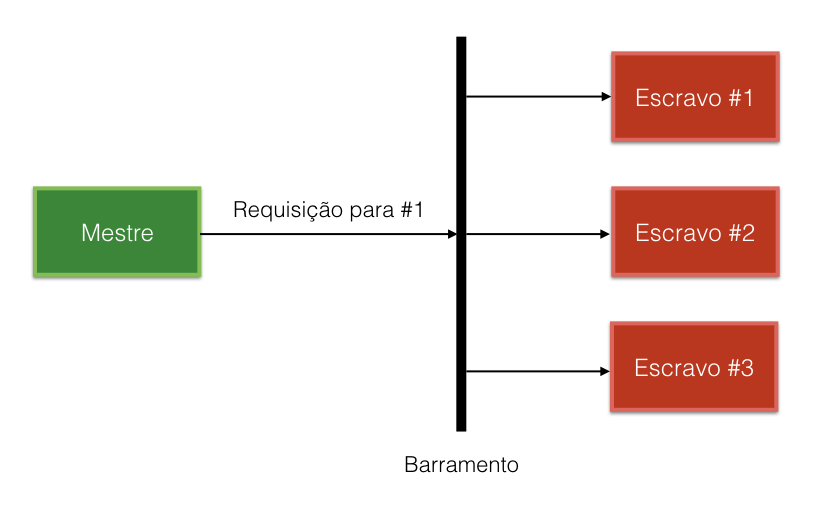
\includegraphics[width=\textwidth,natwidth=1024,natheight=768]{assets/images/modbus-req-1.png}
                \caption{Requisição MODBUS do mestre para o escravo}
                \label{fig:modbus-req-1}
        \end{center}
\end{figure}

Como uma rede pode ter N escravos, cada escravo possui um endereço atribuído. O mestre envia a requisição para o barramento e todos os escravos a recebem, porém somente o endereçado responderá. Há também a opção de se fazer um broadcast - endereço 0 - onde todos escravos recebem a requisição, porém nesse caso nenhum escravo deve responde-lá.

Vale notar que em uma rede MODBUS-RTU há somente um mestre, enquanto em uma rede MODBUS-TCP é possível que cada mestre seja um escravo, e vice-versa.

\begin{figure}[H]
        \begin{center}
                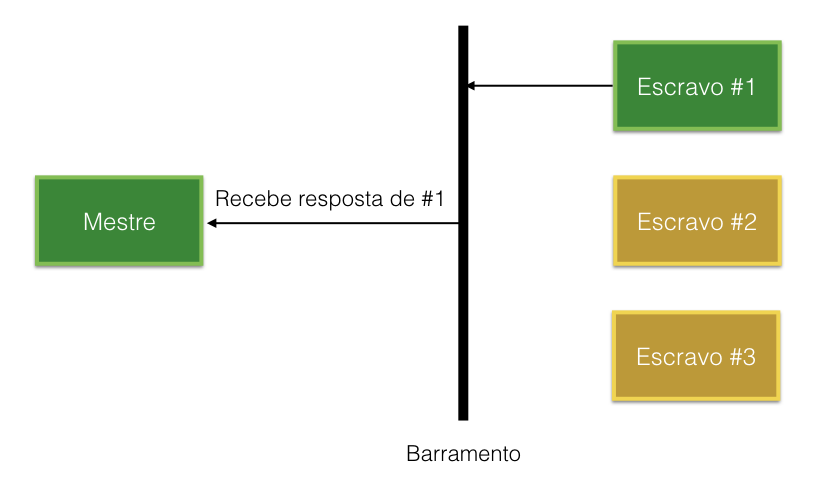
\includegraphics[width=\textwidth,natwidth=1024,natheight=768]{assets/images/modbus-req-2.png}
                \caption{Resposta MODBUS do escravo para o mestre}
                \label{fig:modbus-req-2}
        \end{center}
\end{figure}

\subsection{Mapa de Memória}

Toda requisição realizada pelo mestre endereçará um dado no mapa de memória do dispositivo escravo, sendo que tal mapa de memória normalmente deve ser indicado por uma documentação. Os dados requisitados podem possuir quatro tipos distintos:

\begin{itemize}
  \item \textit{Input}: dado binário que permite apenas leitura
  \item \textit{Coil}: dado binário que permite leitura e escrita
  \item \textit{Input Register}: registrador com 16 bits (inteiro) que permite apenas leitura
  \item \textit{Holding} Register: registrador com 16 bits (inteiro) que permite leitura e escrita
\end{itemize}

Para a realização de operações nesse mapa de memória, o mestre precisa informar nas suas requisições um \textit{function code}. Este indicará qual dado deseja-se requisitar e se será executada uma operação de leitura ou escrita. A tabela \ref{table:modbus-funccodes} mostra os mais comuns, porém existem mais códigos, aos quais podem ser usados para diagnósticos e entre outras funções.

\begin{table}[]
\centering
\caption{Function codes / Operações do MODBUS}
\label{table:modbus-funccodes}
\begin{tabular}{@{}ll@{}}
\toprule
\textbf{Operação}              & \textbf{Function code} \\ \midrule
Leitura de Coils               & 1                      \\
Escrita em 1 Coils             & 5                      \\
Escrita em N Coils             & 15                     \\
Leitura de Inputs              & 2                      \\
Leitura de Input Registers     & 4                      \\
Leitura de Holding Registers   & 3                      \\
Escrita em 1 Holding Register  & 6                      \\
Escrita em N Holding Registers & 16                     \\ \bottomrule
\end{tabular}
\end{table}

\subsection{Envio de informações}

Cada modo possui alguma diferença, porém o meio que as informações são organizadas e enviadas é o mesmo. Na imagem a seguir, é possível observar que em ambas implementações é necessária a definição de um \textit{FCode (function code)}. Logo após vem o campo \textit{Data}, onde devem ser indicado o endereço inicial do mapa de memória, quantos registradores deseja-se requisitar e quais dados serão escritos (no caso de escrita).

\begin{figure}[H]
        \begin{center}
                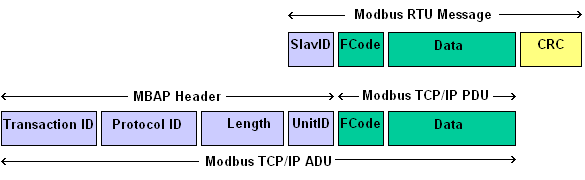
\includegraphics[width=\textwidth,natwidth=585,natheight=180]{assets/images/modbus-frame.png}
                \caption{Frame de Comunicação MODBUS}
                \label{fig:modbus-frame}
        \end{center}
\end{figure}

Como pode-se notar, somente no MODBUS-RTU há o SlavID (endereço), já que os dispositivos MODBUS-TCP são endereçados por seus IPs. O campo CRC é um dado que permite checar se o pacote obtido possui ou não algum erro. Como o protocolo TCP/IP já possui um meio para isso, tal campo não é incluído na requisição.

Esse formato de envio de informações é mantido tanto para requisição quanto para resposta, sendo que as respostas sempre possuem o mesmo \textit{function code} da requisição. Caso diferir, provavelmente ocorreu um erro e este pode ser processado pelo mestre posteriormente.

\section{WSDL e SOAP}

O WSDL \cite{w3c-spec-wsdl} permite descrever serviços web por meio de um arquivo \ac{XML}. É possível definir os \textit{endpoints} - pontos de entrada para requisições - com o que devem retornar e o que devem receber como parâmetros. Isso permite que um serviço web seja desenvolvido por uma equipe que, posteriormente, exporta um WSDL descrevendo de maneira fácil quais são seus endpoints, facilitando a criação de clientes ou servidores compatíveis com o serviço.

Os arquivos WSDL definem suas interfaces em SOAP \cite{w3c-spec-soapspec}, um protocolo que permite trocas de informações entre clientes e servidores de forma padronizada. Ele é baseado em XML e é montado em três partes:
\begin{itemize}
  \item Envolpe: identifica o que é a mensagem e como processá-la
  \item Cabeçalho: define informações extras sobre a mensagem
  \item Corpo: define o procedimento a ser chamado e os dados de sua resposta
\end{itemize}

Como ele foi idealizado em XML, ele é facilmente processado por qualquer linguagem de programação, o que garante uma boa portabilidade.
